% Created by tikzDevice version 0.9 on 2015-12-16 01:29:16
% !TEX encoding = UTF-8 Unicode
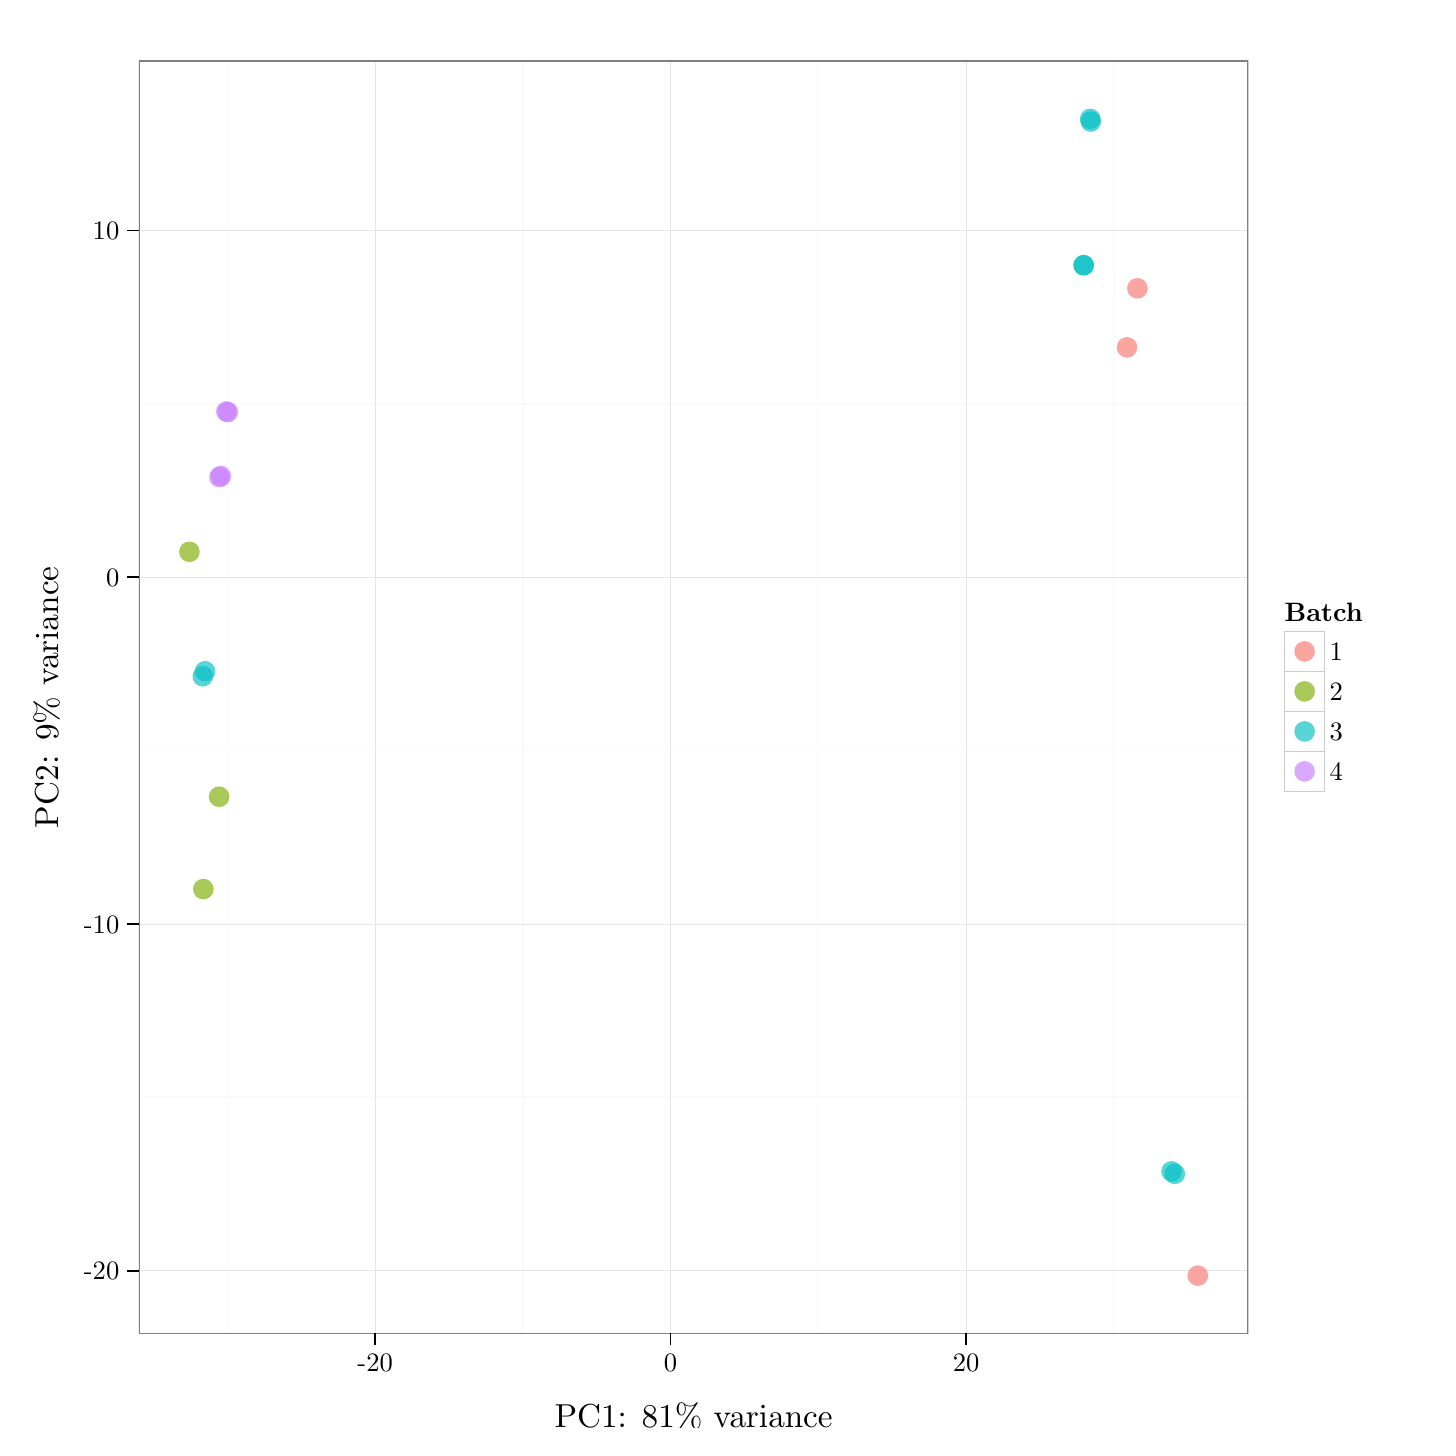
\begin{tikzpicture}[x=1pt,y=1pt]
\definecolor{fillColor}{RGB}{255,255,255}
\path[use as bounding box,fill=fillColor,fill opacity=0.00] (0,0) rectangle (505.89,505.89);
\begin{scope}
\path[clip] (  0.00,  0.00) rectangle (505.89,505.89);
\definecolor{drawColor}{RGB}{255,255,255}
\definecolor{fillColor}{RGB}{255,255,255}

\path[draw=drawColor,line width= 0.6pt,line join=round,line cap=round,fill=fillColor] (  0.00,  0.00) rectangle (505.89,505.89);
\end{scope}
\begin{scope}
\path[clip] ( 40.22, 34.03) rectangle (441.05,493.85);
\definecolor{fillColor}{RGB}{255,255,255}

\path[fill=fillColor] ( 40.22, 34.03) rectangle (441.05,493.85);
\definecolor{drawColor}{gray}{0.98}

\path[draw=drawColor,line width= 0.6pt,line join=round] ( 40.22,119.38) --
	(441.05,119.38);

\path[draw=drawColor,line width= 0.6pt,line join=round] ( 40.22,244.68) --
	(441.05,244.68);

\path[draw=drawColor,line width= 0.6pt,line join=round] ( 40.22,369.97) --
	(441.05,369.97);

\path[draw=drawColor,line width= 0.6pt,line join=round] ( 72.17, 34.03) --
	( 72.17,493.85);

\path[draw=drawColor,line width= 0.6pt,line join=round] (178.94, 34.03) --
	(178.94,493.85);

\path[draw=drawColor,line width= 0.6pt,line join=round] (285.71, 34.03) --
	(285.71,493.85);

\path[draw=drawColor,line width= 0.6pt,line join=round] (392.48, 34.03) --
	(392.48,493.85);
\definecolor{drawColor}{gray}{0.90}

\path[draw=drawColor,line width= 0.2pt,line join=round] ( 40.22, 56.73) --
	(441.05, 56.73);

\path[draw=drawColor,line width= 0.2pt,line join=round] ( 40.22,182.03) --
	(441.05,182.03);

\path[draw=drawColor,line width= 0.2pt,line join=round] ( 40.22,307.32) --
	(441.05,307.32);

\path[draw=drawColor,line width= 0.2pt,line join=round] ( 40.22,432.62) --
	(441.05,432.62);

\path[draw=drawColor,line width= 0.2pt,line join=round] (125.56, 34.03) --
	(125.56,493.85);

\path[draw=drawColor,line width= 0.2pt,line join=round] (232.33, 34.03) --
	(232.33,493.85);

\path[draw=drawColor,line width= 0.2pt,line join=round] (339.10, 34.03) --
	(339.10,493.85);
\definecolor{fillColor}{RGB}{124,174,0}

\path[fill=fillColor,fill opacity=0.65] ( 63.48,194.62) circle (  3.73);

\path[fill=fillColor,fill opacity=0.65] ( 69.19,227.99) circle (  3.73);
\definecolor{fillColor}{RGB}{199,124,255}

\path[fill=fillColor,fill opacity=0.65] ( 72.37,366.95) circle (  3.73);

\path[fill=fillColor,fill opacity=0.65] ( 71.78,367.21) circle (  3.73);

\path[fill=fillColor,fill opacity=0.65] ( 69.28,343.47) circle (  3.73);

\path[fill=fillColor,fill opacity=0.65] ( 69.80,343.90) circle (  3.73);
\definecolor{fillColor}{RGB}{124,174,0}

\path[fill=fillColor,fill opacity=0.65] ( 58.44,316.49) circle (  3.73);
\definecolor{fillColor}{RGB}{0,191,196}

\path[fill=fillColor,fill opacity=0.65] ( 64.10,273.33) circle (  3.73);

\path[fill=fillColor,fill opacity=0.65] ( 63.28,271.50) circle (  3.73);
\definecolor{fillColor}{RGB}{248,118,109}

\path[fill=fillColor,fill opacity=0.65] (422.83, 54.94) circle (  3.73);
\definecolor{fillColor}{RGB}{0,191,196}

\path[fill=fillColor,fill opacity=0.65] (413.32, 92.62) circle (  3.73);

\path[fill=fillColor,fill opacity=0.65] (414.51, 91.73) circle (  3.73);
\definecolor{fillColor}{RGB}{248,118,109}

\path[fill=fillColor,fill opacity=0.65] (397.24,390.37) circle (  3.73);
\definecolor{fillColor}{RGB}{0,191,196}

\path[fill=fillColor,fill opacity=0.65] (384.15,471.97) circle (  3.73);

\path[fill=fillColor,fill opacity=0.65] (383.95,472.94) circle (  3.73);
\definecolor{fillColor}{RGB}{248,118,109}

\path[fill=fillColor,fill opacity=0.65] (400.99,411.70) circle (  3.73);
\definecolor{fillColor}{RGB}{0,191,196}

\path[fill=fillColor,fill opacity=0.65] (381.56,420.04) circle (  3.73);

\path[fill=fillColor,fill opacity=0.65] (381.59,420.04) circle (  3.73);
\definecolor{drawColor}{gray}{0.50}

\path[draw=drawColor,line width= 0.6pt,line join=round,line cap=round] ( 40.22, 34.03) rectangle (441.05,493.85);
\end{scope}
\begin{scope}
\path[clip] (  0.00,  0.00) rectangle (505.89,505.89);
\definecolor{drawColor}{RGB}{0,0,0}

\node[text=drawColor,anchor=base east,inner sep=0pt, outer sep=0pt, scale=  0.96] at ( 33.11, 53.42) {-20};

\node[text=drawColor,anchor=base east,inner sep=0pt, outer sep=0pt, scale=  0.96] at ( 33.11,178.72) {-10};

\node[text=drawColor,anchor=base east,inner sep=0pt, outer sep=0pt, scale=  0.96] at ( 33.11,304.02) {0};

\node[text=drawColor,anchor=base east,inner sep=0pt, outer sep=0pt, scale=  0.96] at ( 33.11,429.32) {10};
\end{scope}
\begin{scope}
\path[clip] (  0.00,  0.00) rectangle (505.89,505.89);
\definecolor{drawColor}{RGB}{0,0,0}

\path[draw=drawColor,line width= 0.6pt,line join=round] ( 35.95, 56.73) --
	( 40.22, 56.73);

\path[draw=drawColor,line width= 0.6pt,line join=round] ( 35.95,182.03) --
	( 40.22,182.03);

\path[draw=drawColor,line width= 0.6pt,line join=round] ( 35.95,307.32) --
	( 40.22,307.32);

\path[draw=drawColor,line width= 0.6pt,line join=round] ( 35.95,432.62) --
	( 40.22,432.62);
\end{scope}
\begin{scope}
\path[clip] (  0.00,  0.00) rectangle (505.89,505.89);
\definecolor{drawColor}{RGB}{0,0,0}

\path[draw=drawColor,line width= 0.6pt,line join=round] (125.56, 29.77) --
	(125.56, 34.03);

\path[draw=drawColor,line width= 0.6pt,line join=round] (232.33, 29.77) --
	(232.33, 34.03);

\path[draw=drawColor,line width= 0.6pt,line join=round] (339.10, 29.77) --
	(339.10, 34.03);
\end{scope}
\begin{scope}
\path[clip] (  0.00,  0.00) rectangle (505.89,505.89);
\definecolor{drawColor}{RGB}{0,0,0}

\node[text=drawColor,anchor=base,inner sep=0pt, outer sep=0pt, scale=  0.96] at (125.56, 20.31) {-20};

\node[text=drawColor,anchor=base,inner sep=0pt, outer sep=0pt, scale=  0.96] at (232.33, 20.31) {0};

\node[text=drawColor,anchor=base,inner sep=0pt, outer sep=0pt, scale=  0.96] at (339.10, 20.31) {20};
\end{scope}
\begin{scope}
\path[clip] (  0.00,  0.00) rectangle (505.89,505.89);
\definecolor{drawColor}{RGB}{0,0,0}

\node[text=drawColor,anchor=base,inner sep=0pt, outer sep=0pt, scale=  1.20] at (240.64,  0) {PC1: 81\% variance};
\end{scope}
\begin{scope}
\path[clip] (  0.00,  0.00) rectangle (505.89,505.89);
\definecolor{drawColor}{RGB}{0,0,0}

\node[text=drawColor,rotate= 90.00,anchor=base,inner sep=0pt, outer sep=0pt, scale=  1.20] at ( 11,263.94) {PC2: 9\% variance};
\end{scope}
\begin{scope}
\path[clip] (  0.00,  0.00) rectangle (505.89,505.89);
\definecolor{fillColor}{RGB}{255,255,255}

\path[fill=fillColor] (449.92,225.64) rectangle (484.98,302.23);
\end{scope}
\begin{scope}
\path[clip] (  0.00,  0.00) rectangle (505.89,505.89);
\definecolor{drawColor}{RGB}{0,0,0}

\node[text=drawColor,anchor=base west,inner sep=0pt, outer sep=0pt, scale=  0.96] at (454.19,291.34) {\bfseries Batch};
\end{scope}
\begin{scope}
\path[clip] (  0.00,  0.00) rectangle (505.89,505.89);
\definecolor{drawColor}{gray}{0.80}
\definecolor{fillColor}{RGB}{255,255,255}

\path[draw=drawColor,line width= 0.6pt,line join=round,line cap=round,fill=fillColor] (454.19,273.27) rectangle (468.64,287.73);
\end{scope}
\begin{scope}
\path[clip] (  0.00,  0.00) rectangle (505.89,505.89);
\definecolor{fillColor}{RGB}{248,118,109}

\path[fill=fillColor,fill opacity=0.65] (461.42,280.50) circle (  3.73);
\end{scope}
\begin{scope}
\path[clip] (  0.00,  0.00) rectangle (505.89,505.89);
\definecolor{drawColor}{gray}{0.80}
\definecolor{fillColor}{RGB}{255,255,255}

\path[draw=drawColor,line width= 0.6pt,line join=round,line cap=round,fill=fillColor] (454.19,258.82) rectangle (468.64,273.27);
\end{scope}
\begin{scope}
\path[clip] (  0.00,  0.00) rectangle (505.89,505.89);
\definecolor{fillColor}{RGB}{124,174,0}

\path[fill=fillColor,fill opacity=0.65] (461.42,266.05) circle (  3.73);
\end{scope}
\begin{scope}
\path[clip] (  0.00,  0.00) rectangle (505.89,505.89);
\definecolor{drawColor}{gray}{0.80}
\definecolor{fillColor}{RGB}{255,255,255}

\path[draw=drawColor,line width= 0.6pt,line join=round,line cap=round,fill=fillColor] (454.19,244.37) rectangle (468.64,258.82);
\end{scope}
\begin{scope}
\path[clip] (  0.00,  0.00) rectangle (505.89,505.89);
\definecolor{fillColor}{RGB}{0,191,196}

\path[fill=fillColor,fill opacity=0.65] (461.42,251.59) circle (  3.73);
\end{scope}
\begin{scope}
\path[clip] (  0.00,  0.00) rectangle (505.89,505.89);
\definecolor{drawColor}{gray}{0.80}
\definecolor{fillColor}{RGB}{255,255,255}

\path[draw=drawColor,line width= 0.6pt,line join=round,line cap=round,fill=fillColor] (454.19,229.91) rectangle (468.64,244.37);
\end{scope}
\begin{scope}
\path[clip] (  0.00,  0.00) rectangle (505.89,505.89);
\definecolor{fillColor}{RGB}{199,124,255}

\path[fill=fillColor,fill opacity=0.65] (461.42,237.14) circle (  3.73);
\end{scope}
\begin{scope}
\path[clip] (  0.00,  0.00) rectangle (505.89,505.89);
\definecolor{drawColor}{RGB}{0,0,0}

\node[text=drawColor,anchor=base west,inner sep=0pt, outer sep=0pt, scale=  0.96] at (470.45,277.20) {1};
\end{scope}
\begin{scope}
\path[clip] (  0.00,  0.00) rectangle (505.89,505.89);
\definecolor{drawColor}{RGB}{0,0,0}

\node[text=drawColor,anchor=base west,inner sep=0pt, outer sep=0pt, scale=  0.96] at (470.45,262.74) {2};
\end{scope}
\begin{scope}
\path[clip] (  0.00,  0.00) rectangle (505.89,505.89);
\definecolor{drawColor}{RGB}{0,0,0}

\node[text=drawColor,anchor=base west,inner sep=0pt, outer sep=0pt, scale=  0.96] at (470.45,248.29) {3};
\end{scope}
\begin{scope}
\path[clip] (  0.00,  0.00) rectangle (505.89,505.89);
\definecolor{drawColor}{RGB}{0,0,0}

\node[text=drawColor,anchor=base west,inner sep=0pt, outer sep=0pt, scale=  0.96] at (470.45,233.83) {4};
\end{scope}
\end{tikzpicture}
